\chapter{GoogLeNet}
{
\label{chap:googlenet}
本研究でマルチFPGA上に実装するアプリケーションであるGoogLeNetについて説明する.
GoogleNetは畳込みニューラルネットワーク(CNN: Convolutional Neural Network)のモデルの1つである.
まずCNNの基本的な演算について説明する
\section{Convolutional Neural Network}
\label{sec:cnn}
2012年のILSVRC()で登場したAlexNetによりCNNは特に画像認識や物体検出の分野で優れた識別精度をマークしたことから世界で注目されるようになった,
%Neural Networkの説明
\subsection{Neural Network}
\label{sec:nn}
ニューラルネットワークは動物の神経ニューロンが接続され、神経物質が伝搬されるように演算モジュールを層として複数、結合していく。
演算ネットワークでは神経物質の代わりに例えば画像における画素値のような入力ベクトルの演算結果を伝搬していく。
ニューラルネットワーク及び機械学習では2つの演算フェーズ、学習と推論がある。
学習では教師データ(識別された画像)をもとに各演算層のパラメータを決定する、
推論では学習で得たパラメータを用いて、入力値(未識別の画像)から演算(入力画像の識別)を行う。
本研究では推論アルゴリズムにフォーカスしたアクセラレータを実装するので推論演算で用いられるアルゴリズムについて説明する
\subsection{Convolution}
\label{sec:conv}
CNNはその名前にも含まれているように式で表される畳み込み演算と呼ばれる行列の積和演算がその主なアルゴリズムである.
CNNでは各層の演算結果を次の層の入力値として受け渡す。これを特徴マップと呼ぶ。
特徴マップは畳み込み層や全結合層で重みフィルタと呼ばれる学習結果から得られる行列と積和演算が行われる
式で畳み込み演算、マックスプーリング、全結合の演算を示す
% conv
\begin{eqnarray}
	output(x, y)^{i} = input(x, y)^{i} / (k + \alpha \sum_{j=max(0, i-n/2)}^{min(N-1, i+n/2)} (a^j_{x, y})^2)^\beta
\end{eqnarray}
% max pool
\begin{eqnarray}
	output(x, y)^{i} = max(input(i, j) | x-k <= i <= x+k, y-k <= j <= y+k)
\end{eqnarray}
% full connect
\begin{eqnarray}
  output(i) = bias(i) + \sum_{j=0}^{N} weight(i, j) * input(j)
\end{eqnarray}

これらの演算を各層で処理し伝搬していき出力されるという構造をとっている.
CNNでは多くのネットワークモデルでこの畳込み層が主である。
\section{GoogLeNet}
\label{sec:googlenet}
GoogLeNetは2014年のILSVRCで最高精度をマークしたCNNのモデルの一つである.構成要素は上述の畳み込み演算,プーリング処理などが主であるという点においてはAlexNetなどと
違いはないが,それぞれの層の接続の仕方,層の深さが異なる,AlexNet, GoogLeNetそれぞれについて図にその全体像を示す

\begin{figure}[h]
  \centering
  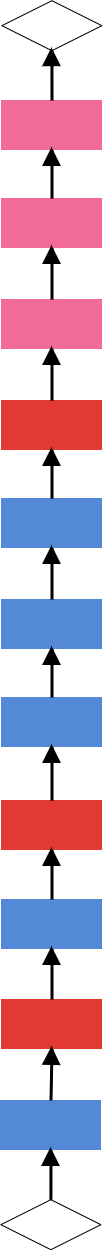
\includegraphics[width=12cm]{./chap2/fig/alexnet.pdf}
  \caption{AlexNetのアーキテクチャ}
  \label{fig:alexnet}
\end{figure}

\begin{figure}[h]
  \centering
  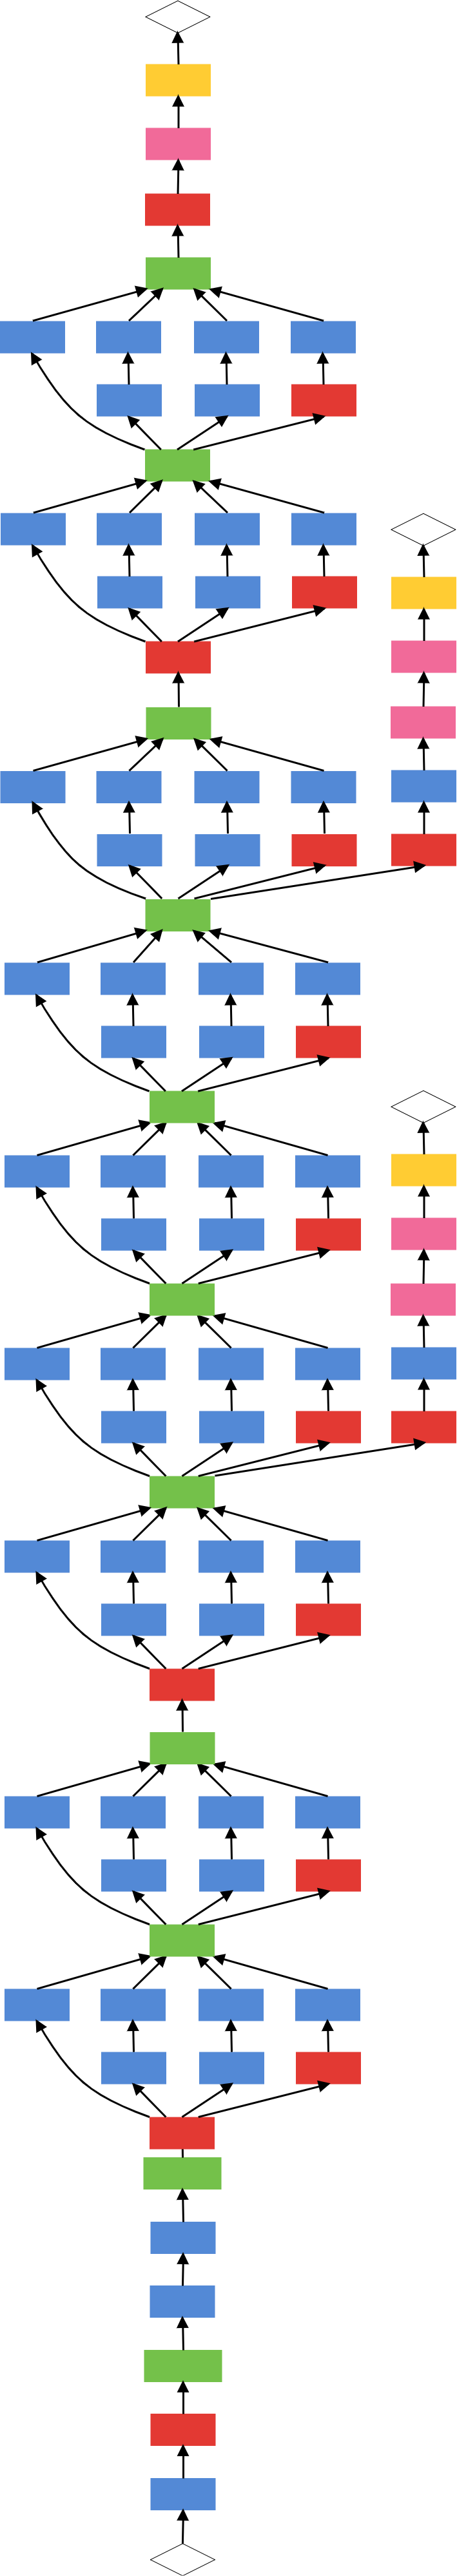
\includegraphics[width=12cm]{./chap2/fig/googlenet.pdf}
  \caption{GoogLeNetのアーキテクチャ}
  \label{fig:googlenet}
\end{figure}
両者を比較すると,GoogLeNetのほうが,層がより深くなっていること,さらに横に広がっていることがわかる.
GoogLeNetは層を深くする代わりにそのフィルタサイズを小さくすることで,計算量,メモリアクセスを減らすように設計されている.
〇〇の研究によると一つの大きなフィルタによる畳込みよりも複数の小さなフィルタによる畳込みのほうがより高い精度を出すことができるとされている.
さらにGoogLeNetでは横に広がった複数の層をInception層と名付け,これを複数層重ねる設計をしている.

\section{Inception}
\label{sec:inception}
Inception層は次の図で示される(これは図の一部を拡大したものと同じである)
\begin{figure}[h]
  \centering
  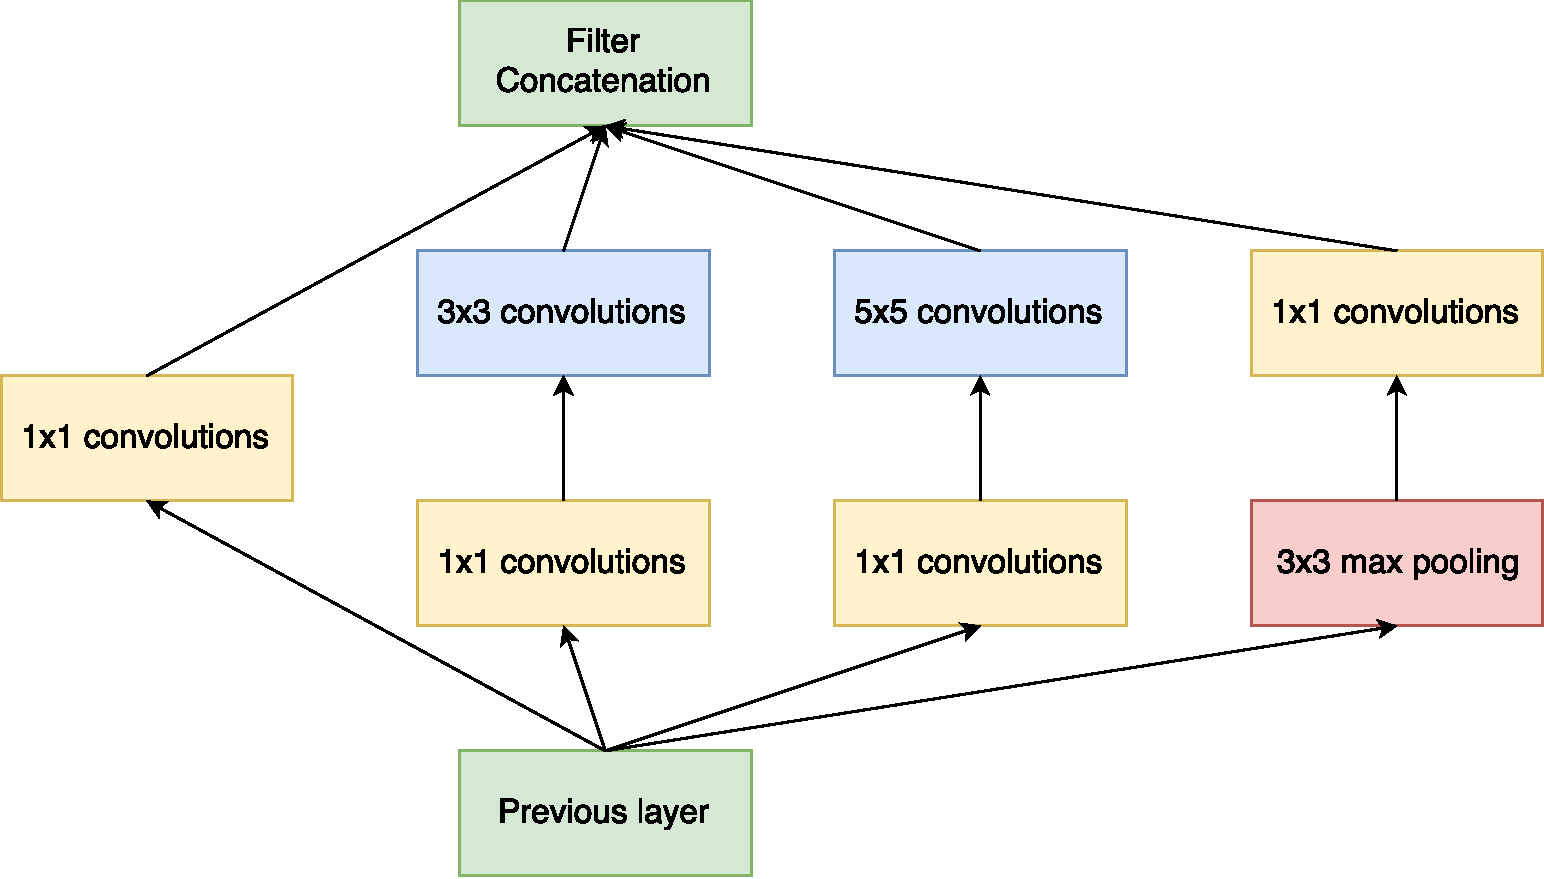
\includegraphics[width=12cm]{./chap2/fig/inception.pdf}
  \caption{Inception層}
  \label{fig:inception}
\end{figure}
これを見ると横に広がった層の中で1*1convと記されている層がある.この層ではサイズ1のフィルターを用いて,畳込み演算を行っている.
この層は,次元削減を行っている.これは入力チャネル(入力行列の深さ)に対して少ない層のフィルタを畳み込み演算することでその深さを
削減する,これによって計算量が減るだけでなく,精度向上が実現できる.
Inception層の出力の手前のDepthConcat層は横に広がった層のそれぞれの出力結果を図○のように深さ方向に結合することで
一つの行列として出力値にまとめる処理を行っている.
\begin{figure}[h]
  \centering
  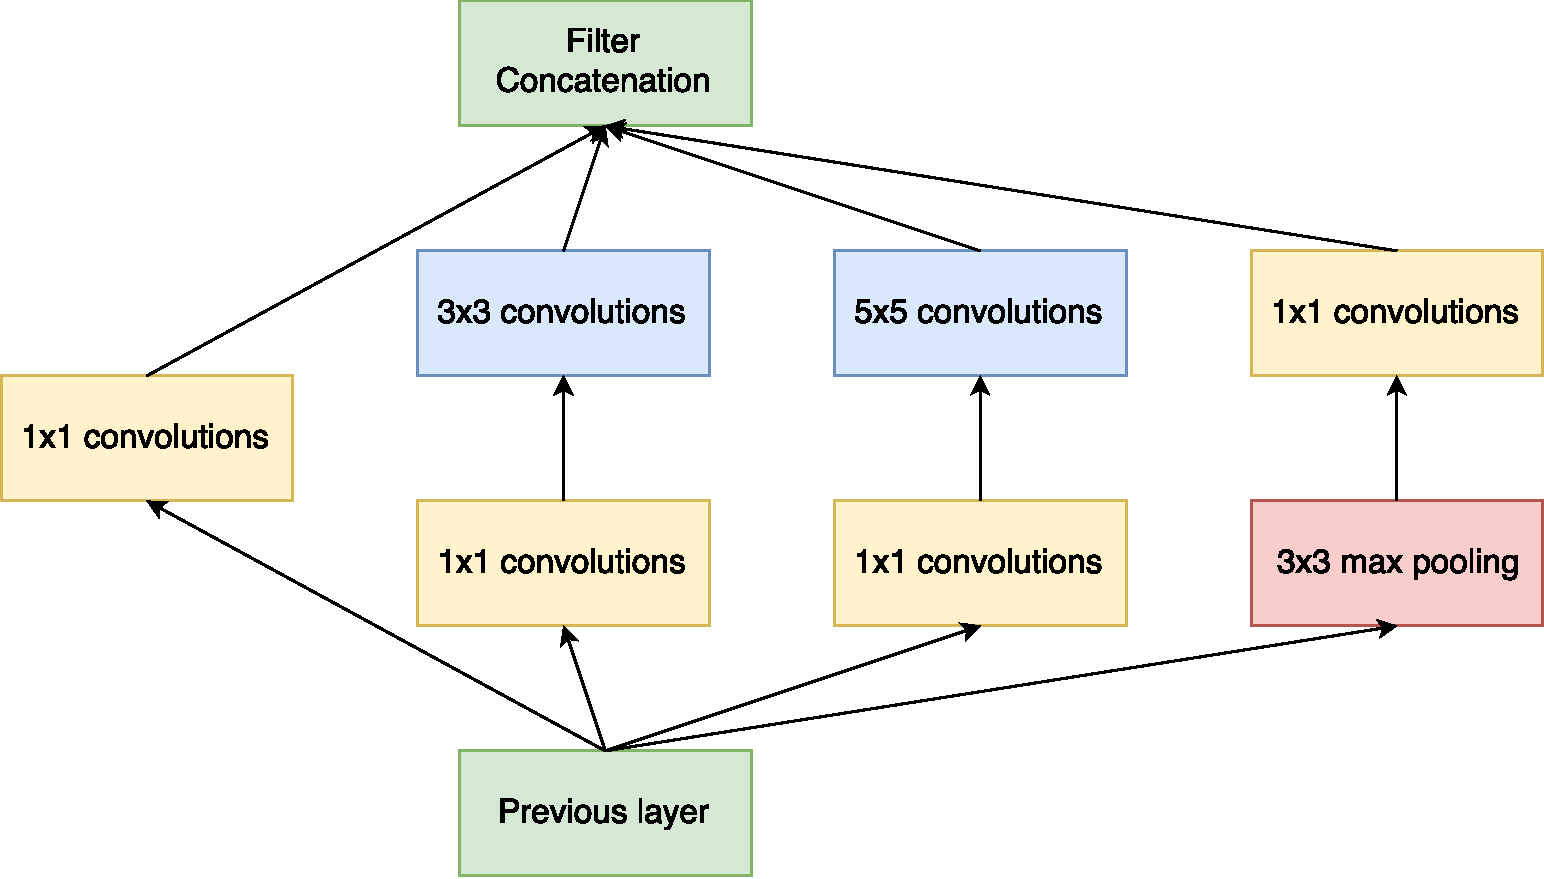
\includegraphics[width=12cm]{./chap2/fig/inception.pdf}
  \caption{Inception層}
  \label{fig:inception}
\end{figure}
この特徴的なInception層を積層していくことで,GoogLeNetは構成される.表○にGoogLeNetでの各層で必要なパラメータ数をまとめる.

\begin{table}[ht]
 \begin{center}
  \caption{GoogLeNetの各層の詳細なパラメータ}
   \begin{tabular}{|c|c|c|c|c|c|c|} \hline
     層 & 入力fm N & 出力fm M & サイズ(R,C) & カーネルK & ストライドS & パディング \\ \hline
     CONV1 & 3 & 96 & 55 & 11 & 4 & 0 \\
     NORM1 & 96 & 96 & 55 & - & - & - \\
     POOL1 & 96 & 96 & 27 & 3 & 2 & - \\
     CONV2 & 96 & 256 & 27 & 5 & 1 & 2 \\
     NORM2 & 256 & 256 & 27 & - & - & - \\
     POOL2 & 256 & 256 & 27 & 3 & 2 & - \\
     CONV3 & 256 & 384 & 13 & 3 & 1 & 1\\
     CONV4 & 384 & 384 & 13 & 3 & 1 & 1\\
     CONV5 & 384 & 256 & 13 & 3 & 1 & 1\\
     POOL5 & 256 & 256 & 6 & 3 & 2 & - \\
     FC6 & 9216 & 4096 & - & - & - & - \\
     FC7 & 4096 & 4096 & - & - & - & - \\
     FC8 & 4096 & 1000 & - & - & - & - \\ \hline
  \end{tabular}
  \label{googlenet_params}  
 \end{center}
\end{table}

この表を見るとAlecNetに見られるような全結合層がないことがわかる.GoogLeNetでは高い認識精度を保ったまま,計算量の多い全結合層を
削除することで全体の計算量を減らしている.
}